% Generado por analysis/src/tablas/apendices.py — no editar a mano.
\begin{figure}[!htbp]
\centering
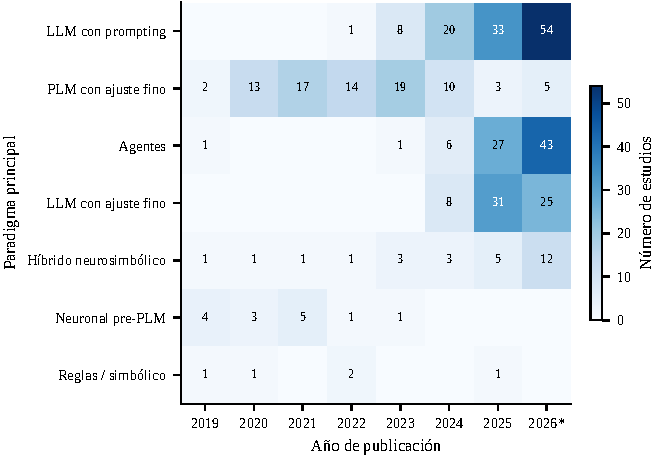
\includegraphics[width=0.8\textwidth]{pi0_paradigma_anio}
\caption{Paradigma técnico principal de los estudios incluidos por año (n = 389; un código por estudio con la precedencia del formulario). *2026: año parcial.}
\label{fig:pi0_paradigma_anio}
\end{figure}

\begin{figure}[!htbp]
\centering
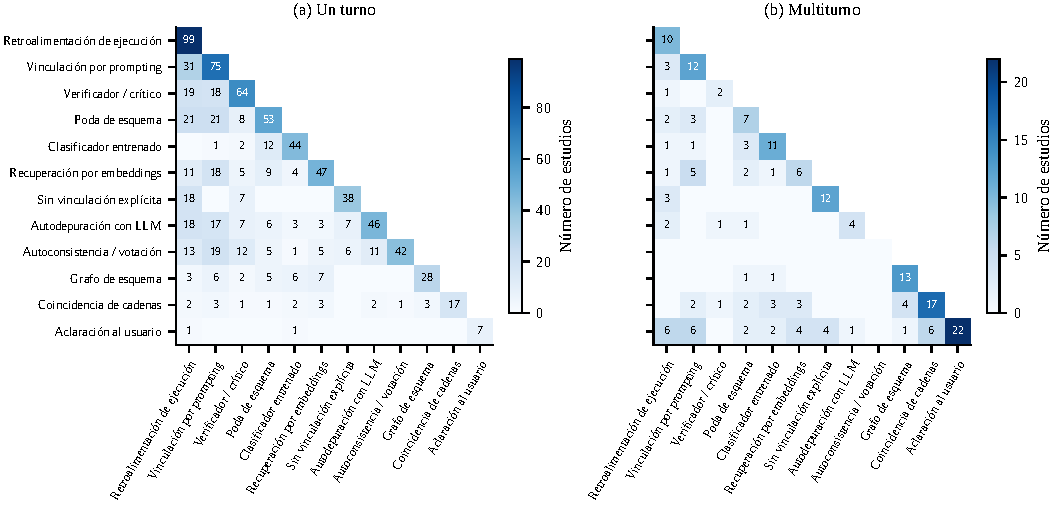
\includegraphics[width=0.8\textwidth]{bib_coocurrencia_tecnicas}
\caption{Coocurrencia de técnicas de vinculación de esquemas (PI3) y de autocorrección (PI4) en un mismo estudio: (a) un turno; (b) multiturno. Diagonal: estudios que usan la técnica; celdas bajo la diagonal: estudios que combinan ambas. Las doce técnicas más frecuentes. Análisis exploratorio.}
\label{fig:bib_coocurrencia_tecnicas}
\end{figure}

